\subsection{Valid decorated posets}
\label{sec:valid_decor}

\begin{lemma}
  \label{lem:no_empty_dec}
  Let $\theta$ a causal trace and let $t_1:M_1\overset{m_1,p_1}{\Rightarrow}N_1$, $t_2:M_2\overset{m_2,p_2}{\Rightarrow}N_2$ be two transitions such that there exists $\spa$ with $t_1\prec ^{\spa} t_2$ or $t_1\dashv^{\spa} t_2$. Then $\spa$ is not empty.
\end{lemma}
\begin{proof}
  It follows from the definition of positive influence (\autoref{def:pos_infl}).
\end{proof}

\begin{lemma}
  \label{lem:pairs_for_influence}
  Let $\theta$ a causal trace and let $t_1:M_1\overset{m_1,p_1}{\Rightarrow}N_1$, $t_2:M_2\overset{m_2,p_2}{\Rightarrow}N_2$ be two transitions such that there exists $\spa:L_1\remb O\lemb L_2$ that commutes in the diagram below:
  \[
  \begin{tikzpicture} %[scale=0.8]
      \node (o) at (0,-1) {\(O\)};
      \node (l1) at (-1,0) {\(L_1\)};
      \node (l2) at (1,0) {\(L_2\)};
      \node (m1) at (-1,1) {\(M_1\)};
      \node (m2) at (1,1) {\(M_2\)};
      \draw [-{Stealth[left]}] (m1) -- (m2);
      \draw [->] (o) -- (l1);
      \draw [->] (o) -- (l2);
      \draw [->] (l1) -- (m1);
      \draw [->] (l2) -- (m2);
    \end{tikzpicture}
    \]
    Let $t_3:M_3\overset{m_3,p_3}{\Rightarrow}N_3$ be a transition such that there exists $\spa_1:R_3\remb O_1\lemb L_1$ with $t_3\prec^{\spa_1}t_1$ and $O\emb O_1$ such that the diagram below commutes:
    \[
    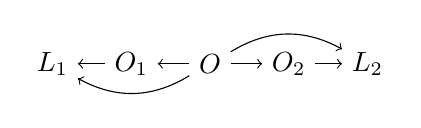
\begin{tikzpicture} %[scale=0.8]
      \node (o) at (0,0) {\(O\)};\
      \node (o1) at (-1,0) {\(O_1\)};
      \node (l1) at (-2,0) {\(L_1\)};
      \node (o2) at (1,0) {\(O_2\)};
      \node (l2) at (2,0) {\(L_2\)};
      \draw [->] (o) -- (o1);
      \draw [->] (o1) -- (l1);
      \draw [->] (o) to [bend left] (l1);
      \draw [->] (o) -- (o2);
      \draw [->] (o2) -- (l2);
      \draw [->] (o) to [bend left] (l2);
    \end{tikzpicture}
    \]
    Then there exists $\spa_2:R_3\remb O_2\lemb L_2$ with $t_3\prec^{\spa_2}t_2$ and $O\emb O_2$ such that the diagram above commutes.
\end{lemma}

\begin{lemma}
  \label{lem:constraint_pos_meet}
  Let $\theta$ a causal trace and let $t_1:M_1\overset{m_1,p_1}{\Rightarrow}N_1$, $t_2:M_2\overset{m_2,p_2}{\Rightarrow}N_2$ and $t_3:M_3\overset{m_3,p_3}{\Rightarrow}N_3$ be three transitions in $\theta$. Let $p_i = L_i\remb K_i \lemb R_i$ be the three rules, for $i\in\{1,2,3\}$.
  Moreover, let $\spa_1:R_1\remb O_1\lemb L_3$ and $\spa_2:R_2\remb O_2\lemb L_3$ be two spans such that $t_1\prec^{\spa_1}_{\theta} t_3$ and $t_2\prec^{\spa_2}_{\theta} t_3$.
     Let $O_1\remb O\lemb O_2$ be the pullback of the span $O_1\lemb L_3 \remb O_2$. Then one of the following holds:
    \begin{itemize}
    \item either there exists the morphisms $O\emb K_1$ and $O\emb K_2$ that commute in the diagram below. In this case~\autoref{lem:pairs_for_influence} holds for $t_1$, $t_2$ and the span $L_1\remb O\lemb L_2$.

    \item or there exists the morphism $O\emb K_1$ but no morphism $O\emb K_2$ that commutes. Then there exists $\spa':R_2\remb O'\lemb L_1$, with $\spa\subseteq \spa'$ for which $t_2\prec^{\spa'}_{\theta} t_1$.
    \end{itemize}
   \[
    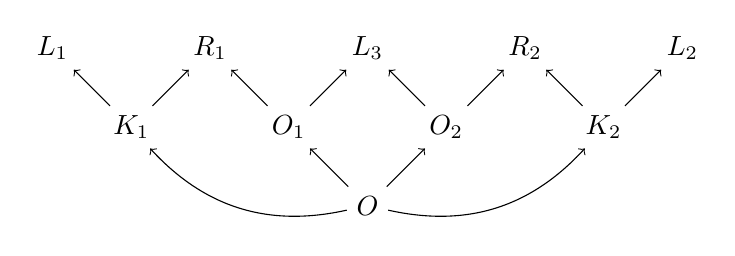
\begin{tikzpicture} %[scale=0.8]
      \node (o) at (0,-1) {\(O\)};
      \node (r3) at (0,1) {\(L_3\)};
      \node (o1) at (-1,0) {\(O_1\)};
      \node (o2) at (1,0) {\(O_2\)};
      \node (r1) at (-2,1) {\(R_1\)};
      \node (r2) at (2,1) {\(R_2\)};
      \node (l1) at (-4,1) {\(L_1\)};
      \node (l2) at (4,1) {\(L_2\)};
      \node (k1) at (-3,0) {\(K_1\)};
      \node (k2) at (3,0) {\(K_2\)};
      \draw [->] (o) -- (o1);
      \draw [->] (o) -- (o2);
      \draw [->] (o1) -- (r3);
      \draw [->] (o2) -- (r3);
      \draw [->] (o1) -- (r1);
      \draw [->] (o2) -- (r2);
      \draw [->] (k1) -- (r1);
      \draw [->] (k2) -- (r2);
      \draw [->] (k1) -- (l1);
      \draw [->] (k2) -- (l2);
      \draw [->] (o) to [bend left] (k1);
      \draw [->] (o) to [bend right] (k2);
    \end{tikzpicture}
    \]
\end{lemma}
\begin{proof}
  We have two similar subcases: $t_1$ precedes $t_2$ in $\theta$ or the other way around. We consider the first case and have the following diagram:
  \[
  \begin{tikzpicture} %[scale=0.8]
    \node (o1) at (2,0) {\(O_1\)};
    \node (o2) at (6,0) {\(O_2\)};
    \node (o) at (3.5,-1) {\(O\)};
    \node (m1) at (-2,3) {\(M_1\)};
    \node (n1) at (0,3) {\(N_1\)};
    \node (n2) at (4,3) {\(N_2\)};
    \node (m2) at (2,3) {\(M_2\)};
    \node (m3) at (6,3) {\(M_3\)};
    \node (r1) at (0,1) {\(R_1\)};
    \node (k1) at (-1,1) {\(K_1\)};
    \node (l1) at (-2,1) {\(L_1\)};
    \node (l2) at (2,1) {\(L_2\)};
    \node (k2) at (3,1) {\(K_2\)};
    \node (r2) at (4,1) {\(R_2\)};
    \node (l3) at (6,1) {\(L_3\)};
    \draw [->] (o) -- (o1);
    \draw [->] (o) -- (o2);
    \draw [->] (o1) -- (r1);
    \draw [->] (o1) to [bend right] (l3);
    \draw [->] (o2) -- (r2);
    \draw [->] (o2) -- (l3);
    \draw [->] (r1) --  (n1);
    \draw [->] (l2) --  (m2);
    \draw [->] (l1) --  (m1);
    \draw [->] (r2) --  (n2);
    \draw [->] (l3) --  (m3);
    \draw [-{Stealth[left]}] (m1) -- (n1);
    \draw [-{Stealth[left]}] (n1) --  (m2);
    \draw [-{Stealth[left]}] (m2) -- (n2);
    \draw [-{Stealth[left]}] (n2) -- (m3);
    \draw [-{Stealth[left]}] (n1) to [bend left] (m3);
    \draw [->] (k1) -- (r1);
    \draw [->] (k1) -- (l1);
    \draw [->] (k2) -- (r2);
    \draw [->] (k2) -- (l2);
  \end{tikzpicture}
  \]
  where every path commutes. It follows from the~\autoref{def:dep}, and from obtaining $O$ from a pullback.
  Let $x\in O$ be an edge or a node. For simplifying the notations, we denote $x_G$ for the mapping of $x$ to an element of $G$ whenever there is a path from $O$ to $G$.

  As $x\in O$ it implies there exists $x_{O_1}$ and $x_{O_2}$ that both map to $x_{L_3}$.
  From $t_1\prec^{\spa_1}t_3$, there exists $x_{R_1}$ and $x_{M_3}$ such that $x_{L_3}$ and $x_{R_1}$ map to $x_{M_3}$. But then there exists $x_{M_2}$ and $x_{N_2}$ such that $x_{O_2}$ maps to $x_{N_2}$. It implies the existance of $x_{K_2}$. As this holds for all $x\in O$, we have that $O\emb K_2$.

  We distinguish between two subcases:
  \begin{itemize}
  \item Suppose that there is a morphism $O\emb K_1$ that makes the diagram commute and then~\autoref{lem:pairs_for_influence} holds.

  \item Otherwise, there exists $x\in O$ and $x_{R_1}$ such that there is no $x_{K_1}$ with $r(x_{K_1})=x_{R_1}$. But as $x\in O$, from above, we have that there exists $x_{K_2}$ and hence $x_{L_2}$. Therefore there exists at least one positive influence $\spa'$ containing the mapping of $x$ to $x_{R_1}$ and $x$ to $x_{L_2}$ and with $x_{R_1}\notin K_1$. Hence $t_1\prec^{\spa'}_{\theta} t_2$.
  \end{itemize}
\end{proof}

Inutuitively, \autoref{lem:constraint_pos_meet} says that if two events cannot \emph{produce} the same resource. It covers the constraints on decorating positive meets in \autoref{def:constraints_poset}. The lemmas for the rest of the cases are similar.

\begin{example}
  For the following rules:
  \[
  r_1:\varepsilon \Rightarrow A,B \qquad r_2: \varepsilon \Rightarrow A,C \qquad r_3: A,B,C \Rightarrow D
  \]
  there is a trace where $t_1<t_3$ and $t_2<t_3$, however both cannot produce $A$:
    \[
    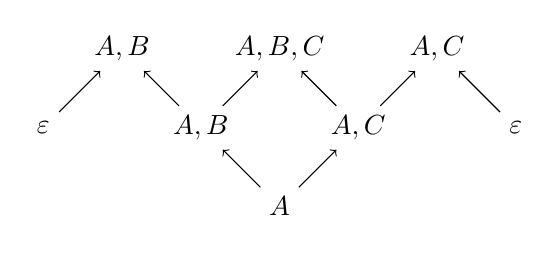
\begin{tikzpicture} %[scale=0.8]
      \node (o) at (0,-1) {\(A\)};
      \node (r3) at (0,1) {\(A,B,C\)};
      \node (o1) at (-1,0) {\(A,B\)};
      \node (o2) at (1,0) {\(A,C\)};
      \node (r1) at (-2,1) {\(A,B\)};
      \node (r2) at (2,1) {\(A,C\)};
      \node (k1) at (-3,0) {\(\varepsilon\)};
      \node (k2) at (3,0) {\(\varepsilon\)};
      \draw [->] (o) -- (o1);
      \draw [->] (o) -- (o2);
      \draw [->] (o1) -- (r3);
      \draw [->] (o2) -- (r3);
      \draw [->] (o1) -- (r1);
      \draw [->] (o2) -- (r2);
      \draw [->] (k1) -- (r1);
      \draw [->] (k2) -- (r2);
    \end{tikzpicture}
    \]
\end{example}

\begin{lemma}
  \label{prop:app_constraints_poset}
  For any causal trace $\theta$, $\mathsf{decoration\_of\_trace}(\theta)$ is a valid decorated poset.
\end{lemma}
\begin{proof}
  It follows from~\autoref{lem:no_empty_dec} and~\autoref{lem:lem:constraint_pos_meet}.
\end{proof}
